\documentclass{article}
\usepackage{NotesTeXV3}

%% 
\allowdisplaybreaks
\raggedbottom

%%
\title{CIE 327 - Probability and Stochastic Processes}
\author{SalahDin A. Rezk}
\affiliation{Zewail City of Science and Technology}
\emailAdd{s-salahdin.rezk@zewailcity.edu.eg}
\date{\today}
\abstract{
    Student's notes for the Communication and Information Engineering Probability Course by Prof. Samy Soliman at Zewail City of Science and Technology in the Fall 24/25 semester. The notes are based on the lectures and the textbook \textit{Probability, Random Variables, and Stochastic Processes} by Athanasios Papoulis and S. Unnikrishna Pillai. Other references include \textit{Probability and Statistics for Engineers and Scientists} by Ronald E. Walpole and Raymond H. Myers; and \textit{Modern Digital and Analog Communication Systems} by B. P. Lathi.and Zhi Ding. The notes cover the basics of probability theory, random variables, and stochastic processes.
}


\begin{document}

\maketitle

\part{Probability Theory}
\section{Introduction}

Probability applications are everywhere, from weather forecasting to aerospace engineering. It is a mathematical tool to model uncertainty. 

\begin{definition}[Random Experiment]
An experiment with an uncertain outcome.
\end{definition}

\begin{definition}[Sample Space]
The set of all possible outcomes.
\end{definition}

\begin{example}[Heads or Tails]
The sample space is $\{H, T\}$.
\end{example}

\begin{example}[Rolling a Die]
The sample space is $\{1, 2, 3, 4, 5, 6\}$.
\end{example}

\begin{example}[Point on a Circle]
The sample space is $S = \{(x, y) \mid x^2 + y^2 \leq 5\}$.
\end{example}

\begin{remark}
The number of elements in a sample space may be finite, infinite, countable, or uncountable.
\end{remark}

\begin{marginfigure}
  \centering
  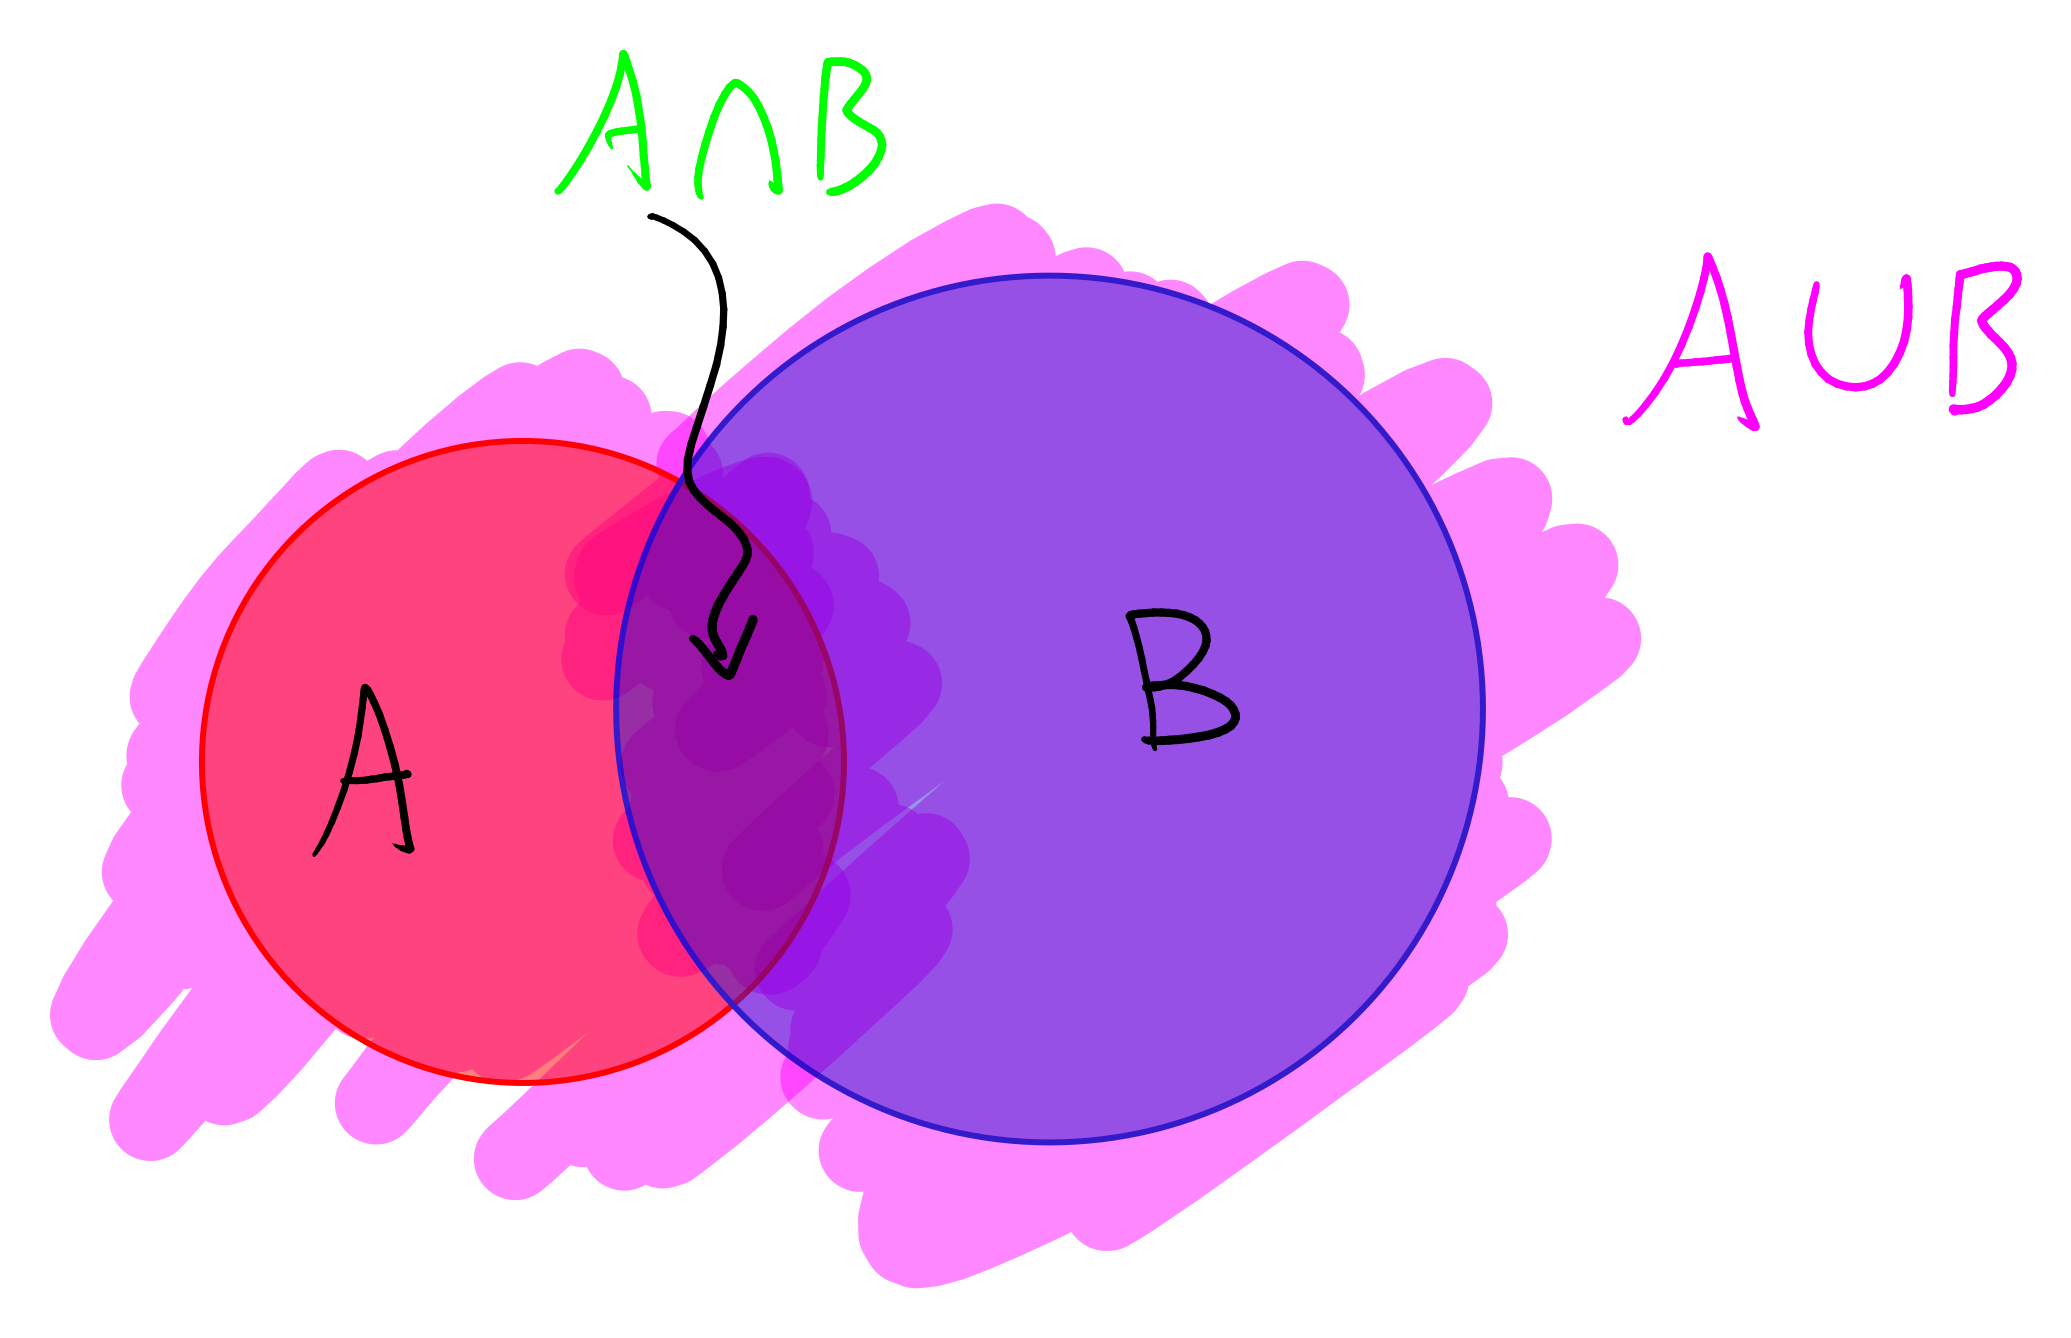
\includegraphics[width=\textwidth]{images/image_20250108_001846.png}
  \caption{Example of Unions and Intersections on events \( A \) and \( B \).}
  \label{fig:unions_intersections}
\end{marginfigure}

\begin{definition}[Event]
A subset of the sample space.
\end{definition}

\begin{definition}[Complement]
The event that is not in $A$, denoted by $A'$.
\end{definition}

\begin{definition}[Union]
An event that is in $A$ or $B$, denoted by $A \cup B$.
\end{definition}

\begin{definition}[Intersection]
An event common to both $A$ and $B$, denoted by $A \cap B$.
\end{definition}

\begin{definition}[Mutually Exclusive/Disjoint]
Two events are mutually exclusive/disjoint if they have no common outcomes, i.e., $A \cap B = \emptyset$.
\label{def:mutually_exclusive}
\end{definition}

\begin{definition}[Venn Diagram]
A diagram that shows the relationships between events. See Figures.
\end{definition}

\begin{marginfigure}
    \centering
    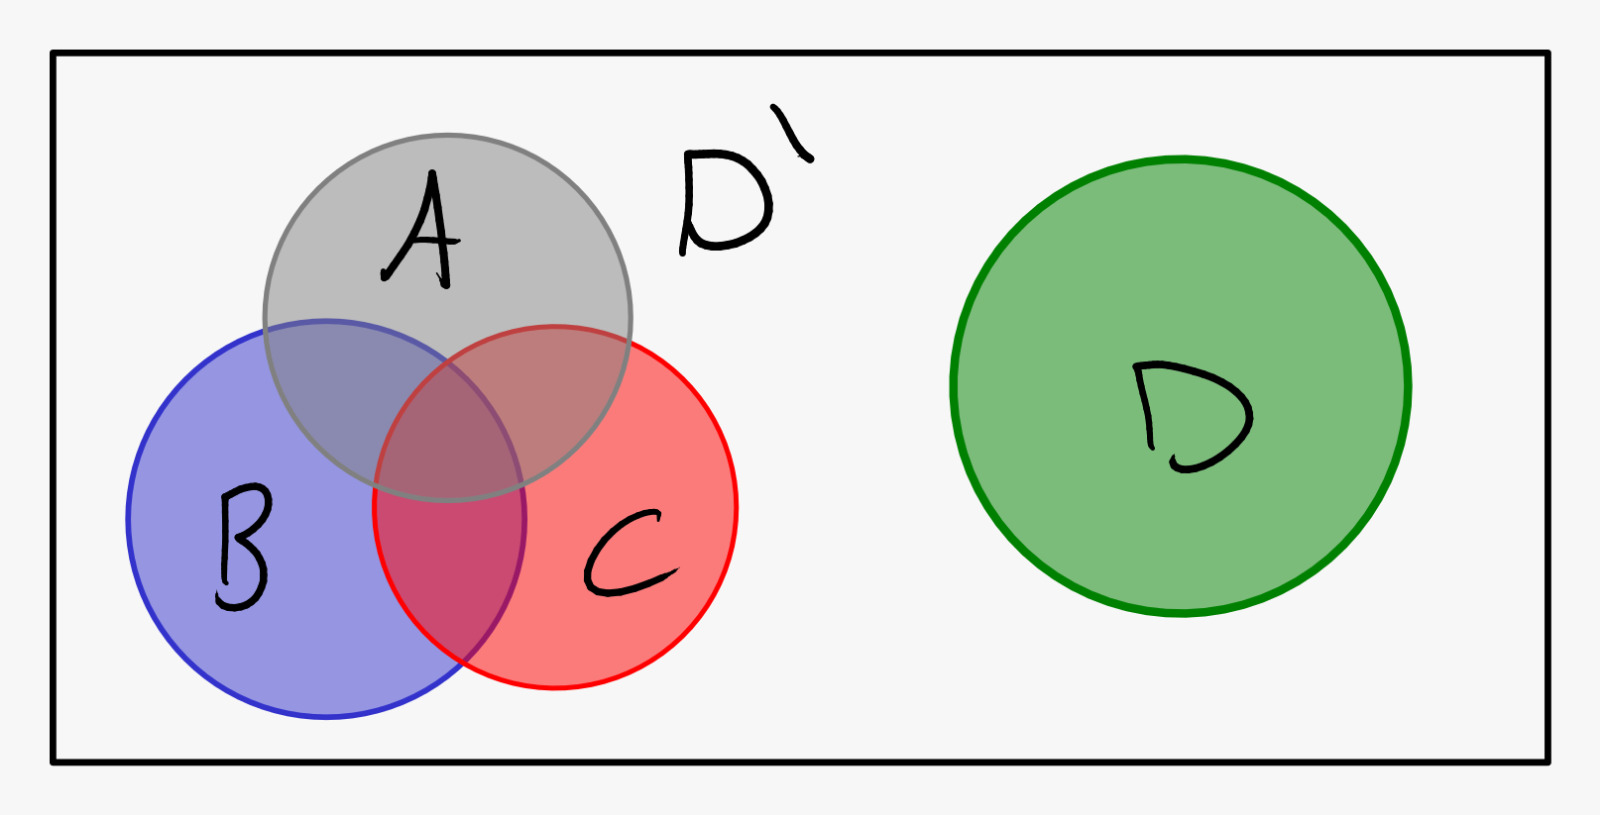
\includegraphics[width=\textwidth]{figures/ven-diagram.jpeg}
    \caption{Venn Diagram for Sample Space \( S \)}
    \label{fig:sample_space}
\end{marginfigure}

\subsection{Some Properties of Events}

\begin{align}
    A \cap \emptyset &= \emptyset \\
    A \cup \emptyset &= A \\
    A \cap A' &= \emptyset \\
    A \cup A' &= S \\
    S' &= \emptyset \\
    (A')' &= A \\
    (A \cup B)' &= A' \cap B' \label{eq:union_prime} \\
    (A \cap B)' &= A' \cup B' \label{eq:intersection_prime}
.\end{align}

\marginnote{Check the Venn Diagram in Figure~\ref{fig:venn_properties} for a visual representation of these properties.}

\begin{proof}[Equation~\ref{eq:union_prime}]
\begin{align*}
    x \in (A \cup B)' &\iff x \notin A \cup B \\
    &\iff x \notin A \text{ and } x \notin B \\
    &\iff x \in A' \text{ and } x \in B' \\
    &\iff x \in A' \cap B'.
\end{align*}
\end{proof}

\begin{proof}[Equation~\ref{eq:intersection_prime}]
\begin{align*}
    x \in (A \cap B)' &\iff x \notin A \cap B \\
    &\iff x \notin A \text{ or } x \notin B \\
    &\iff x \in A' \text{ or } x \in B' \\
    &\iff x \in A' \cup B'.
\end{align*}
\end{proof}

\begin{figure}[htbp]
  \begin{fullpage}
    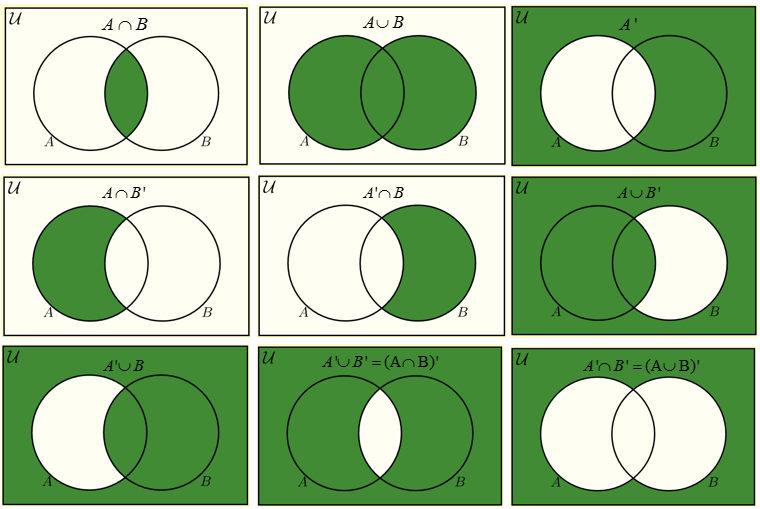
\includegraphics[width=\textwidth]{images/20250108_003400.png}
    \caption{Venn Diagram for some proprieties.}
    \label{fig:venn_properties}
  \end{fullpage}
\end{figure}

\subsection{Axioms of Probability}
\begin{itemize}
    \item $P(A) \in [0, 1]$ for all events $A$.
    \item $P(S) = 1$.
    \item If $A_1, A_2, \ldots$ are mutually exclusive, then $P\left(\bigcup_{i=1}^\infty A_i\right) = \sum_{i=1}^\infty P(A_i)$.
\end{itemize}

\subsection{More Rules}
\begin{align}
  P(A') &= 1 - P(A) \label{eq:complement} \\
    P(A \cup B) &= P(A) + P(B) - P(A \cap B) \\
    P(\varnothing) &= 0
\end{align}

\begin{proof}[Equation~\ref{eq:complement}]
\begin{align*}
    P(A \cup A') &= P(S) = 1 \\
    \intertext{Since $A$ and $A'$ are mutually exclusive (Definition~\ref{def:mutually_exclusive}),}
    P(A) + P(A') &= 1 \\
    P(A') &= 1 - P(A).
\end{align*}
\end{proof}

\newpage
\section{Counting Techniques}

They are used to determine the number of outcomes in a sample space. Helpful for calculating probabilities and will still be useful in later chapters.

\subsection{Multiplication Rule}
\begin{definition}[Multiplication Rule]
If an experiment consists of $n_1$ stages, where the first stage can result in $n_1$ outcomes, the second stage in $n_2$ outcomes, and so on, the total number of outcomes is $n_1 \times n_2 \times \cdots \times n_k = \prod_{i=1}^k n_i$.
\end{definition}

\begin{example}[License Plates]
A license plate consists of 3 letters followed by 3 digits. Total number of plates is $26^3 \times 10^3$.
\end{example}

\begin{definition}[Factorial]
The product of all positive integers up to $n$.
\begin{align*}
    n! &= n \times (n-1) \times \cdots \times 1.
\end{align*}
\end{definition}

\begin{remark}
\begin{itemize}
    \item $0! = 1$.
    \item $n! = n \times (n-1)!$.
\end{itemize}
Factorials are used to calculate permutations and combinations, representing the number of ways to arrange a set of objects.
\end{remark}

\begin{example}[Arranging Professors]
Nine professors are to give talks at a conference, grouped by nationality (3 French, 2 American, 4 Egyptian). In how many ways can their talks be scheduled so that professors of the same nationality follow each other?
\begin{align*}
    \text{Arrange French: } &3! \\
    \text{Arrange American: } &2! \\
    \text{Arrange Egyptian: } &4! \\
    \text{Arrange Nationalities: } &3! \\
    \text{Total: } &3! \times (3! \times 2! \times 4!) = 1728.
\end{align*}
\end{example}

\subsection{Combinatorics}
\begin{definition}[Permutation]
An arrangement of $n$ objects in a specific order.
\begin{align*}
    P(n, r) &= \frac{n!}{(n-r)!}.
\end{align*}
\end{definition}

\begin{proof}[Proof of Permutation Formula]
To arrange $r$ items from $n$ distinct items:
\begin{itemize}
    \item $n$ options for the first position.
    \item $n-1$ for the second.
    \item Continue until $n-r+1$ options for the $r$-th position.
\end{itemize}
Thus,
\begin{align*}
    P(n, r) &= n \times (n-1) \times \cdots \times (n-r+1) \\
    &= \frac{n!}{(n-r)!}.
\end{align*}
\end{proof}

\begin{remark}
\begin{itemize}
    \item If $r=n$, then $P(n, n) = n!$.
    \item If $r=0$, then $P(n, 0) = 1$.
\end{itemize}
\end{remark}

\begin{example}[Seating 5 People]
How many ways can 5 people be seated in a row?
\begin{align*}
    P(5, 5) &= \frac{5!}{(5-5)!} = 5!.
\end{align*}
Thus, there are $5! = 120$ ways.
\end{example}

\begin{definition}[Combination]
    An arrangement of $r$ objects from $n$ objects without considering the order.
    \[
        C(n,r)=\frac{n!}{r!\times (n-r)!}
    .\] 
\end{definition}

\begin{proof}[Combination Formula]
    Number of ways to choose $r$ items from $n$ distinct items without considering the order. First find the number of ways to arrange $r$ items from $n$ distinct items, then divide by the number of ways to arrange the $r$ items. Therefore, the total
    \begin{align*}
        C(n,r) &= \frac{P(n,r)}{P(r,r)} \\
               &= \frac{n!}{r!\times(n-r)!} \times \frac{r!}{r!} \\
               &= \frac{n!}{r!\times(n-r)!}.
    .\end{align*}
\end{proof}

\begin{remark}
    \begin{itemize}
        \item $C(n, r) = C(n, n-r)$.
        \item $C(n, 0) = 1$.
        \item $C(n, 1) = n$.
        \item $C(n, n) = 1$.
    \end{itemize}
\end{remark}

\begin{example}
    An 8-bit codeword is selected at random. What is the probability that it contains at least 3 zero bits?
    \begin{align*}
        T &= \sum^{8}_{i=3} \binom{8}{i} \\
          &= 2^{8}-\sum^{3}_{i=0} \binom{8}{i} \\
          &= 163 \\
        P &= \frac{163}{2^{8} }=0.6367 \\
    .\end{align*}
\end{example}

\subsection{Binomial Theorem}

\begin{definition}[Binomial Theorem]
    \[
        (x+y)^{n}=\sum^{n}_{k=0} \binom{n}{k}x^{n-k}y^{k}
    .\]
\end{definition}

\begin{example}
    Expand $(x+y)^{3}$.
    \begin{align*}
        (x+y)^{3} &= \binom{3}{0}x^{3}y^{0}+\binom{3}{1}x^{2}y^{1}+\binom{3}{2}x^{1}y^{2}+\binom{3}{3}x^{0}y^{3} \\
                  &= x^{3}+3x^{2}y+3xy^{2}+y^{3}.
    \end{align*}
\end{example}

\section{Conditional Probability}

\begin{definition}[Conditional Probability]
The probability of an event \( B \) occurring given that \( A \) has occurred. It is denoted as \( P(B|A) \).
\begin{align}
    P(B|A) &= \frac{P(A \cap B)}{P(A)}; \quad P(A) > 0. \label{eq:conditional} \\
    \intertext{similarly,}
    P(A|B) &= \frac{P(A \cap B)}{P(B)}; \quad P(B) > 0. \nonumber
\end{align}
\label{def:conditional_probability}
\end{definition}

In a Venn Diagram, conditional probability is equivalent to changing the sample space to \( B \) and calculating the probability of \( A \) in this new space. For example, in Figure~\ref{fig:conditional}, \( P(A|B) = \frac{P(A \cap B)}{P(B)} \). Imagine wrapping the space around \( B \) and considering only the outcomes in this new space.

\begin{marginfigure}
    \centering
    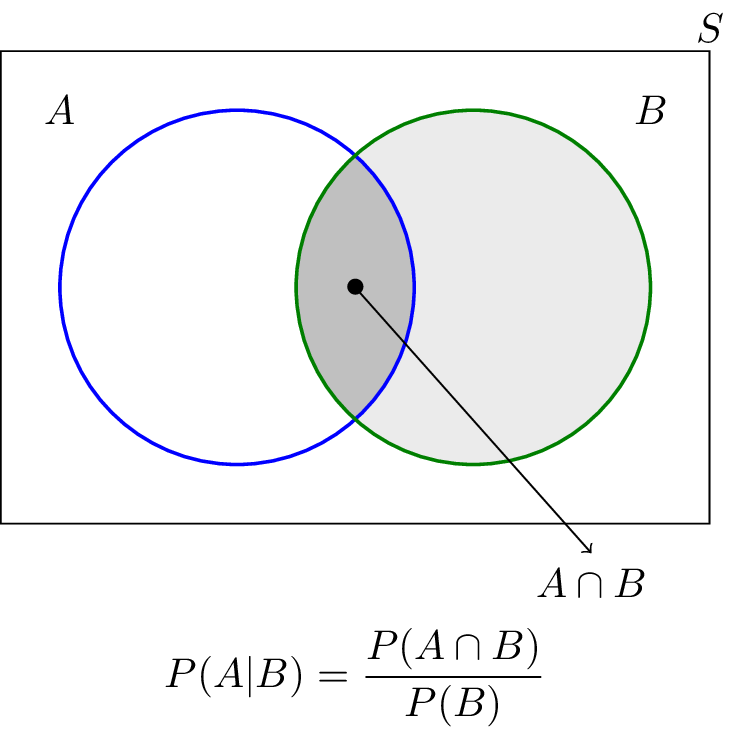
\includegraphics[width=\textwidth]{images/20250110_153104.png}
    \caption{Conditional Probability in a Venn Diagram.}
    \label{fig:conditional}
\end{marginfigure}

\begin{definition}[Independence of Events]
Two events \( A \) and \( B \) are independent if:
\[
    P(B|A) = P(B) \quad \text{or} \quad P(A|B) = P(A)
.\] 
Equivalently:
    \[
    P(A \cap B) = P(A)P(B)
    .\] 
\end{definition}

Independence is not the same as disjointness. Disjoint events are dependent, but independent events are not disjoint. Not related to mutual exclusivity.

\begin{theorem}[General Multiplicative Rule]
For events \( A_1, A_2, \ldots, A_k \):
\begin{align}
    P(A_1 \cap A_2 \cap \cdots \cap A_k) &= P(A_1)P(A_2|A_1)P(A_3|A_1 \cap A_2)\cdots P(A_k|A_1 \cap \cdots \cap A_{k-1}). \\
    P(\bigcap_{i=1}^k A_{i} ) &= \prod_{i=1}^k P(A_i|\bigcap_{j=1}^{i-1} A_j).
\end{align}
If the events are independent:
\begin{align}
    P(A_1 \cap A_2 \cap \cdots \cap A_k) &= P(A_1)P(A_2)\cdots P(A_k).
\end{align}
\label{thm:general_multiplicative_rule}
\end{theorem}

\begin{proof}[General Multiplicative Rule]
    To prove the formula for \( P(A_1 \cap A_2 \cap \cdots \cap A_k) \), we proceed by using the definition of conditional probability iteratively.
    \begin{align*}
        P(A_{1} \cap B_{1}) &= P(B_{1})P(A_{1}|B_{1}) \\
        \intertext{Let \( B_{1} = A_{2} \cap B_{2} \),}
        P(A_{1} \cap A_{2} \cap B_{2}) &= P(A_{2} \cap B_{2})P(A_{1}|A_{2} \cap B_{2}) \\
        &= P(B_{2})P(A_{2}|B_{2})P(A_{1}|A_{2} \cap B_{2}) \\
        \intertext{Since intersection is associative, we can reorder the terms.}
        P(B_{2} \cap A_{2} \cap A_{1}) &= P(B_{2})P(A_{2}|B_{2})P(A_{1}|A_{2} \cap B_{2}) \\
        \intertext{Change of variables,}
        P(A_{1} \cap A_{2} \cap A_{3}) &= P(A_{1})P(A_{2}|A_{1})P(A_{3}|A_{1} \cap A_{2}) \\
        \intertext{Repeat \( k \)-times,}
        P(A_{1} \cap A_{2} \cap \cdots \cap A_{k}) &= P(A_{1})P(A_{2}|A_{1})P(A_{3}|A_{1} \cap A_{2})\cdots P(A_{k}|A_{1} \cap \cdots \cap A_{k-1})
    .\end{align*}
\end{proof}

\begin{theorem}[Total Probability]
If events \( B_1, B_2, \ldots, B_k \) partition the sample space \( S \):
\begin{align}
    P(A) &= \sum_{i=1}^k P(B_i \cap A) = \sum_{i=1}^k P(B_i)P(A|B_i).
\end{align}
\end{theorem}

\begin{marginfigure}
    \centering
    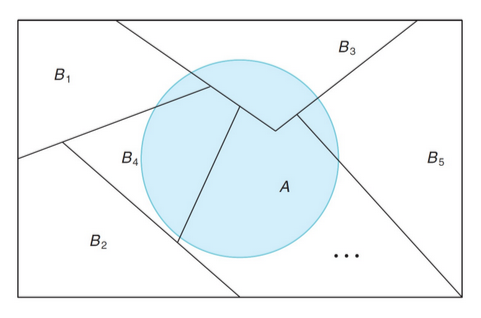
\includegraphics[width=\textwidth]{images/20250110_171204.png}
    \caption{Total Probability in a Venn Diagram.}
    \label{fig:total_probability}
\end{marginfigure}

Total probability is a way to calculate the probability of an event \( A \) by considering all possible ways it can occur. In Figure~\ref{fig:total_probability}, the probability of \( A \) is the sum of the probabilities of \( A \) given each event \( B_i \) times the probability of \( B_i \). We usually trace the path of \( A \) through the events \( B_i \) to calculate the conditional probability using a tree diagram (Figure~\ref{fig:tree_diagram}) to reach the total probability.

\begin{figure}[h]
    \centering
    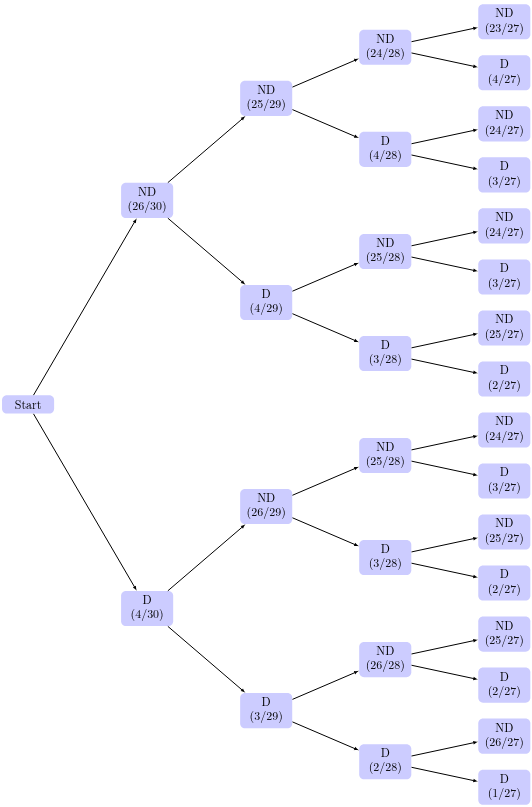
\includegraphics[width=0.65\textwidth, angle=-90]{images/20250110_171731.png}
    \caption{Tree Diagram for Conditional Probability.}
    \label{fig:tree_diagram}
\end{figure}

\begin{theorem}[Bayes' Rule]
If events \( B_1, B_2, \ldots, B_k \) partition the sample space \( S \):
\begin{align}
    P(B_r|A) &= \frac{P(A|B_r)P(B_r)}{\sum_{i=1}^k P(A|B_i)P(B_i)}.
\end{align}
\end{theorem}

\begin{proof}[Bayes' Rule]
\begin{align*}
    \intertext{By the definition of conditional probability \ref{def:conditional_probability},}
    P(B_r|A) &= \frac{P(A \cap B_r)}{P(A)} \\
    \intertext{By the multiplication rule \ref{thm:general_multiplicative_rule},}
    &= \frac{P(A|B_r)P(B_r)}{\sum_{i=1}^k P(A|B_i)P(B_i)}.
\end{align*}
\end{proof}

\part{Random Variables}

\section{Discrete Random Variables}

\subsection{Introduction}
A \textit{discrete random variable (RV)} is a type of variable that can take on a finite or countably infinite set of values. It provides a numerical summary of outcomes from a random experiment.

\begin{example}[Coin Toss]
Consider tossing a coin twice. Define the random variable $X$ as the number of heads observed. The range of $X$ is $\{0, 1, 2\}$.
\end{example}

\begin{example}[Switchboard Calls]
Let $X$ denote the inter-arrival time between calls and $Y$ the number of calls received in a day at a switchboard. The range of $X$ is the set of non-negative real numbers, while the range of $Y$ is the set of non-negative integers.
\end{example}

\subsection{Probability Mass Function (PMF)}
The \textit{probability mass function (PMF)} of a discrete RV $X$ describes the probability of each possible value:
\[
f(x) = P(X = x),
\]
subject to the following properties:
\begin{enumerate}
    \item $f(x) \geq 0$ for all $x$.
    \item $\sum_x f(x) = 1$.
\end{enumerate}

\begin{example}[Defective Computers]
A shipment of 8 microcomputers includes 3 defective units. If a random selection of 2 computers is made, determine the probability distribution of the number of defective computers selected.
\end{example}

\subsection{Cumulative Distribution Function (CDF)}
The \textit{cumulative distribution function (CDF)} of a discrete RV $X$ is given by:
\[
F(x) = P(X \leq x) = \sum_{x_i \leq x} f(x_i),
\]
with the following properties:
\begin{enumerate}
    \item $F(x)$ is non-decreasing.
    \item $F(x) \in [0, 1]$ for all $x$.
\end{enumerate}

\begin{example}[Coin Toss Until a Tail]
A coin is tossed until a tail appears or three attempts are made. Determine the PMF and CDF for the number of tosses required, and sketch their graphs.
\end{example}

\subsection{Expected Value (Mean)}
The \textit{expected value} or \textit{mean} of a discrete RV $X$ is defined as:
\[
\mu = E[X] = \sum_x x f(x).
\]

\begin{example}[Expected Number of Chemists]
A committee of size 2 is randomly selected from a group of 4 chemists and 3 biologists. Compute the expected number of chemists on the committee.
\end{example}

\subsection{Variance}
The \textit{variance} of a discrete RV $X$ measures its spread around the mean:
\[
\sigma^2 = \mathrm{Var}(X) = E[(X - \mu)^2].
\]

\begin{example}[Revenue Comparison]
Two product designs are compared based on revenue:
\begin{itemize}
    \item Design A has a fixed revenue of \$3 million.
    \item Design B has a 30\% chance of yielding \$7 million and a 70\% chance of yielding \$2 million.
\end{itemize}
Calculate the mean and standard deviation for each design.
\end{example}

\subsection{Expected Value of a Function}
For a function $g(X)$ of a discrete RV $X$, the expected value is:
\[
E[g(X)] = \sum_x g(x) f(x).
\]

\begin{example}[Linear Transformation]
Find $E[aX + b]$ for constants $a$ and $b$.
\end{example}

\newpage
\part{Stochastic Processes}

\end{document}
